\documentclass[12pt, a4paper]{article}
\usepackage{a4wide}
\usepackage{graphicx}
\usepackage{float}
\usepackage{hyperref}
\usepackage{listings}
\usepackage[usenames,dvipsnames]{color}

\title{----------------------------------------------------------- \\
        {\bf Programming of Supercomputers WS 12/13}\\ 
        ----------------------------------------------------------- \\ 
        Final report}
\author{Marco Seravalli}
\date{January 24th 2013}

\newcommand{\tab}{\hspace{10mm}}
\newcommand{\draft}[1]{\textcolor{NavyBlue}{#1}}
\newcommand{\hint}[1]{\textcolor{OliveGreen}{{\it#1}}}
         
\begin{document}
  \maketitle

\section{Introduction}
The Programming of Supercomputers laboratory is about understanding how already
applications can be modified and optimized in order to be run efficiently and
effectively on massively parallel machines.

The laboratory is divided into two main parts: the first one is about
understanding how a sequential code can be optimized by acting on the input
phase and on the compilation phase.

The second part is instead more concerned about parallelizing a sequential
Computational Fluid Dynamic application. This process is performed throughout 
four steps (milestones).
\begin{itemize}
  \item In the first phase the domain has to be decomposed using different 
        strategies. First of all a straightforward approach is adopted: here 
        contiguous blocks of elements are assigned to a single processor without
        taking the actual position into account. Afterwards also some advanced
        partitioning algorithms provided by the \verb=metis= library are
        introduced namely \verb=metis-dual= and \verb=metis-nodal=.
  \item The second stage consists in building the communication lists that have 
        to be used for the successive computation part. In this phase also other 
        positioning arrays have to be adapted for being able to respect the 
        correctness of the communication.
  \item The third step involves the actual parallelization of the computational
        loop. This requires to understand how the data within the loop should be
        exchanged during the computation.
  \item The aim of the fourth and last part is the optimization of the code in
        order to be able to deliver a better performing application that
        satisfies some predefined standards. The particular objective in this
        case is to reduce the communication overhead for a specific problem 
        under the threshold of 25\%. 
\end{itemize}

\clearpage

\section{Sequential optimization}
The sequential optimization consists in applying different compiler flags to
the code in order to see the effects produced by those in terms of speedup,
cache hit improvements and floating point operations per second (flops).
Then the optimizations are validated by running the application with different
input files.
In following graphs it is possible to see how the various compiler optimization
affected the execution time (Figure \ref{fig:exec_time}) and the L2 cache miss 
rate (Figure \ref{fig:cache_misses}).
\begin{figure}[h]
  \begin{centering}
    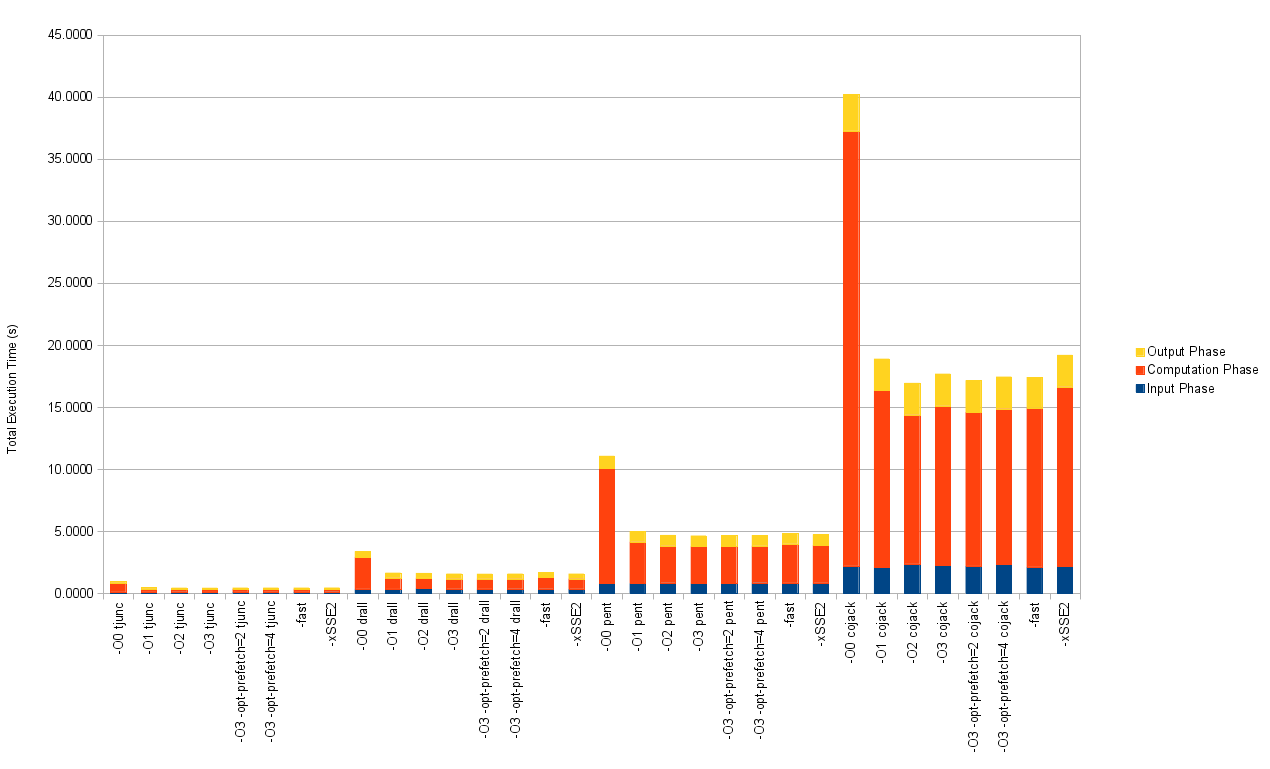
\includegraphics[width=1\textwidth]{figures/exec_time.png}
    \par\end{centering}
  \caption{Execution time for each phase. \label{fig:exec_time}}
\end{figure}

\begin{figure}[h]
  \begin{centering}
    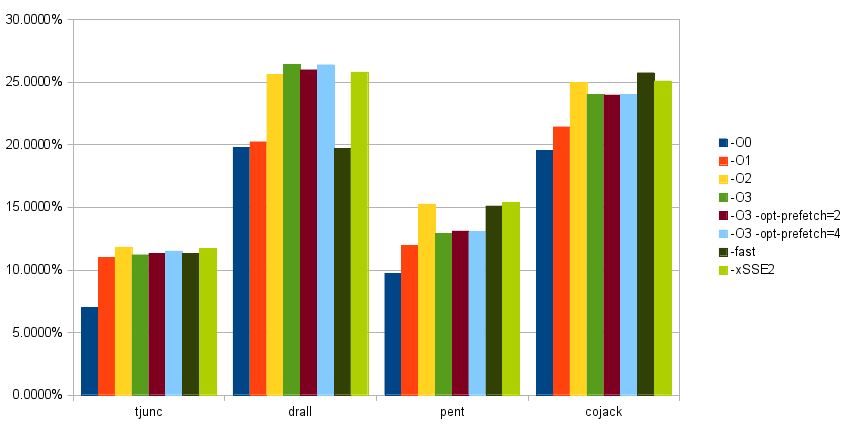
\includegraphics[width=1\textwidth]{figures/cache.png}
    \par\end{centering}
  \caption{L2 cache miss rate. \label{fig:cache_misses}}
\end{figure}

Furthermore, also the file reading phase is modified from text to binary. This 
means that the input files are converted from ASCII values to a binary 
representation.
Also this change provides good speed enhancements to the file reading phase. 
The improvement can be quantified in one order of one order of magnitude. In
Figure \ref{fig:io} it can be seen the execution improvement and how the
it is related to the size of the input file.
\begin{figure}[h]
  \begin{centering}
    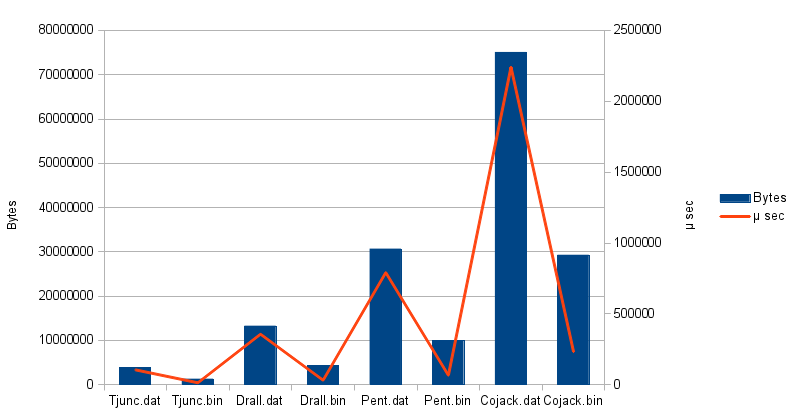
\includegraphics[width=1\textwidth]{figures/io.png}
    \par\end{centering}
  \caption{
    Execution time of the input phase in relation to the input file size. 
    \label{fig:io}
  }
\end{figure}

\clearpage

\section{Benchmark parallelization}

  \subsection*{Data distribution}
  The data are distributed using different partitioning schemes.
  In particular the classical distribution and two different distributions
  offered by the \verb=Metis= partitioning library.

  For the classical distribution the partitioning is performed by splitting the
  domain composed of $n$ cells equally among the computing units $np$ in a
  sequential way, i.e. the first $ \frac{n}{np} $ cells are assigned to the
  first process, then the second set of $ \frac{n}{np} $ sequential cells is
  assigned to the second process and so forth.

  For the two other distributions the whole array containing the cells is passed
  to the functions provided by the \verb=Metis= library. For more information 
  about how the distribution is performed by these functions please refer to
  \href{http://glaros.dtc.umn.edu/gkhome/metis/metis/overview}{Metis Homepage}.

  The partitioning was firstly performed on a single processor, eventually in
  order to decrease the communication among the computing units, this step was
  computed in parallel by every single processor.

  The different partitioning strategies are handled by two different functions
  and for these the code duplication is reduced to the minimum: the partitioning
  functions only perform the strictly necessary tasks. In order to achieve this
  result as mush code as possible is shifted in the calling function.

  \subsection*{Communication model}
  For the communication model send and receive lists have been used in
  particular it has been necessary to guarantee that the received data was
  actually received at the correct position. In addition to that lists for
  knowing how many elements have to be sent and received from each processor are
  initialized as well.

  Once the communications lists are created the global to local index can be
  created from those. The idea for this index is to first to see what elements
  do belong to a specific processor and assign them an incremental number. Then
  during a successive traversal the ghost cells have incrementally numbered.
  The actual implementation can be seen in the following code.

  \begin{verbatim}
// initialise global_local  
int count = 0;
for (int i = 0; i < el_int_glob; ++i) {
    if (part_elems[i] == my_rank) {
        (*global_local)[i] = count;
        ++count;
    } else {
        (*global_local)[i] = -1;
    }
}

for (int i = 0; i < size; ++i) {
    for (int j = 0; j < recv_count[i]; ++j) {
        if ((*global_local)[recv_list[i][j]] == -1) {
            (*global_local)[recv_list[i][j]] = count;
            ++count;
        }
    }
}
  \end{verbatim}

  The reason for such numbering is mainly due to the successive phase the
  building of the local to global index. In this index, we want to have the
  inner elements at the beginning of the array and the ghost cells at the end.
  Since the global to local index holds that specific structure it is
  successively possible to initialize \verb=local_global=  in a single 
  traversal as it can be seen in the following code snippet.

  \begin{verbatim}
// after the initialization of global_local we build up local_global
for (int i = 0; i < el_int_glob; ++i) {
    if (global_local[i] != -1) {
        (*local_global)[global_local[i]] = i;
    }
}
  \end{verbatim}

  After having the indexes set it is also possible to modify the communication 
  lists and the lcc array in order to have the local indexes of the elements. 
  This allows to apply only a minimum amount of changes in the original code.
  A further issue needs to be now solved, the external cells, i.e. the cells
  outside the boundaries. The applications treats all these cells in the very
  same way and their coefficients are always $0$. It follows that all the
  information regarding these elements can be stored in a single position. This
  is performed by making the coefficient arrays one element longer and storing a
  this additional information in the last cell. Of course also lcc needs to be
  modified accordingly, such that all the external cells point to the very same
  position in the coefficient arrays. This change yields to the final form of
  the \verb=local_global_index= that can be seen in Figure \ref{fig:array}.
  \begin{figure}[h]
    \begin{centering}
      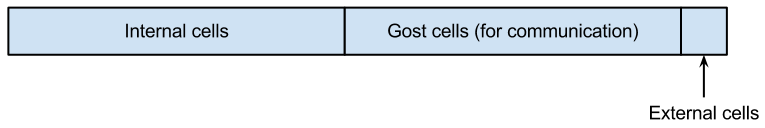
\includegraphics[width=1\textwidth]{figures/array.png}
      \par\end{centering}
    \caption{
      How elements are stored within the local to global index. 
      \label{fig:array}
    }
  \end{figure}


  \subsection*{MPI implementation}
  For the MPI implementation different aspects should be taken into account:
  \begin{itemize}
    \item Point to point operations: the communication among the different
          processors is handled by point to point operations. In such scenario
          every process sends the information only to another processor at a
          time.
    \item Non blocking communication: if blocking point to point communication 
          is used, deadlocks might occur. The reason is that the some processes
          need to send data before being able to receive information, If it
          happens that all processes communicate will all processes (there is a
          clique), it might occur the case that all processes are ready to
          send, but none is ready to receive causing then a deadlock. This can
          be avoided by using non blocking communication. The sending function
          returns immediately even if the data are not actually send. Also for
          the receiving non blocking communication can be exploited. In this
          case the advantage would be that the incoming data from all processes
          can be received in parallel. Eventually, before performing further
          operations on the received and sent data there is the necessity of
          waiting for the communication to be completed.
    \item Indexed data: for sending data indexed data types are adopted. With
          this data type model MPI sends only the necessary elements from the
          correct position for each array. When receiving the data another
          indexed data type should be used instead because the data has to be
          received in the correct positions of the array. In the current
          implementation, there are created send and receive data types for
          every process with whom there is a communication. The building of
          these indexes is performed by using the send and receive lists
          previously created. 
          \begin{verbatim}
for (int i = 0; i < size; ++i) {
    if (send_count[i] > 0) {
        block_len = (int*) calloc(send_count[i], sizeof(int));
        for (int j = 0; j < send_count[i]; ++j) {
            block_len[j] = 1;
        }
        MPI_Type_indexed(send_count[i], 
                         block_len, 
                         send_list[i], 
                         MPI_DOUBLE,
                         &(send_types[i]));
        MPI_Type_commit(&(send_types[i]));
        free(block_len);
    }
    if (recv_count[i] > 0) {
        block_len = (int*) calloc(recv_count[i], sizeof(int));
        for (int j = 0; j < recv_count[i]; ++j) {
            block_len[j] = 1;
        }
        MPI_Type_indexed(recv_count[i],
                         block_len,
                         recv_list[i],
                         MPI_DOUBLE,
                         &(recv_types[i]));
        MPI_Type_commit(&(recv_types[i]));
        free(block_len);
    }
}
          \end{verbatim}
    \item Collective operations: some of the variables of the serial
          implementation are computed taking into account all elements of the
          domain. Of course the parallel code needs to take into account this
          computations and one of the most efficient ways to compute these
          values is via collective operations. In particular for the given
          implementation \verb=MPI_Allreduce=  was adopted. This
          function allows to all the processes to share the result once it is
          computed, hence afterwards no further communication is required.
  \end{itemize}

\clearpage

\section{Performance analysis and tuning}
For this last phase first of all an optimization aim is set, then the code is
analysed using different profiling tools and after the analysis some
modifications are performed in order to reach the predefined objective.

\subsection*{Performance aims}
The major objective of the performance is to reduce the communication overhead
under 25\% for the whole application. 

\subsection*{Profiling}
The code is analyzed using different tools, namely the ScoreP framework in 
collaboration with the PAPI library and the Periscope tool.
ScoreP in particular was used for instrumenting the code and then manually
inspect the outcome through Cube, a visualization tool that allows to scan the
different dimensions of the profiling result.
Periscope was instead employed to automatically find bottlenecks and hot-spots
of the application.

The outcome of the first analysis is that there is particularly high
communication overhead in the initialization part. This is due to the fact that
the partitioning is performed on a process and then distributed to the others.

The computational loop presents some overhead only in the \verb=Allreduce= MPI
function. Small overhead is due to the communication functions \verb=send= and
\verb=recv= because asynchronous communication is adopted since the first
parallelization.

The finalization phase does not present a great overhead because all the data
are communicated only once and the largest amount of time is spent in writing
information on the disk.

\subsection*{Optimization}
The communication overhead in the first part could be overcome by computing 
directly the partitioning on all processes in order to minimize communication. 
Even though in this case more computations are performed, the overall
performance is not affected.

To reduce the communication overhead, all the duplicates from the communication
lists are deleted so that only the needed information was exchanged.

Furthermore in order to be able to overlap communication and computation the
sending and the receiving of data was modified after the initial implementation.
In the first approach the data was communicated at the beginning of the
computational cycle using \verb=IRecv= and \verb=ISend= in that order.

\begin{verbatim}
while ( iter < max_iters ) {
    update the old direc1 values
    receive direc1 values
    send direc1 values
    ...

    update resvec
    ...
}
\end{verbatim}

However in order to be able to perform computation while communicating, 
computation and the sending of \verb=direc1= was moved after the computation of
\verb=resvec=.
This required to rearrange also the first send and the last receive statement as
it can be seen in the following pseudo code.

\begin{verbatim}
update the old direc1 values
send direc1 values

while ( iter < max_iters ) {
    receive direc1 values
    ...

    update resvec
    update the old direc1 values
    send direc1 values
    ...
}

receive direc1 values
\end{verbatim}

Unfortunately, the improvements yield by the optimization step are not directly
visible. One of the possible causes could be the fact that also the reference
code contains asynchronous communication and the optimisations performed to not
lead to significant changes in the adopted concepts.

\subsection*{Scaling results}


\section{Overview}
The lab course proposed an opportunity to approach the parallelization of some
provided code. During the different phases several unexpected challenges had to
be solved. In particular, a careful planning of the data structures and the
communication had been necessary to be able to reach a working solution.

\end{document}

